\chapter{Analyse}


\section{Domäne}

Die Applikation besitzt, wenn man die Daten selbst nicht miteinbezieht, ein relativ simples Domänen-Modell, wie in \cref{fig:pd:domain-model} zu sehen ist. Der Endbenutzer kann mehrere Dateien ablegen oder bereits vorhandene transformieren. Da das Resultat von Dateien oder Transformationen dasselbe ist, werden diese mit dem Oberbegriff Datenpaket\footnote{Im Frontend: ``Package''} versehen.

\begin{figure}[H]
    \centering
    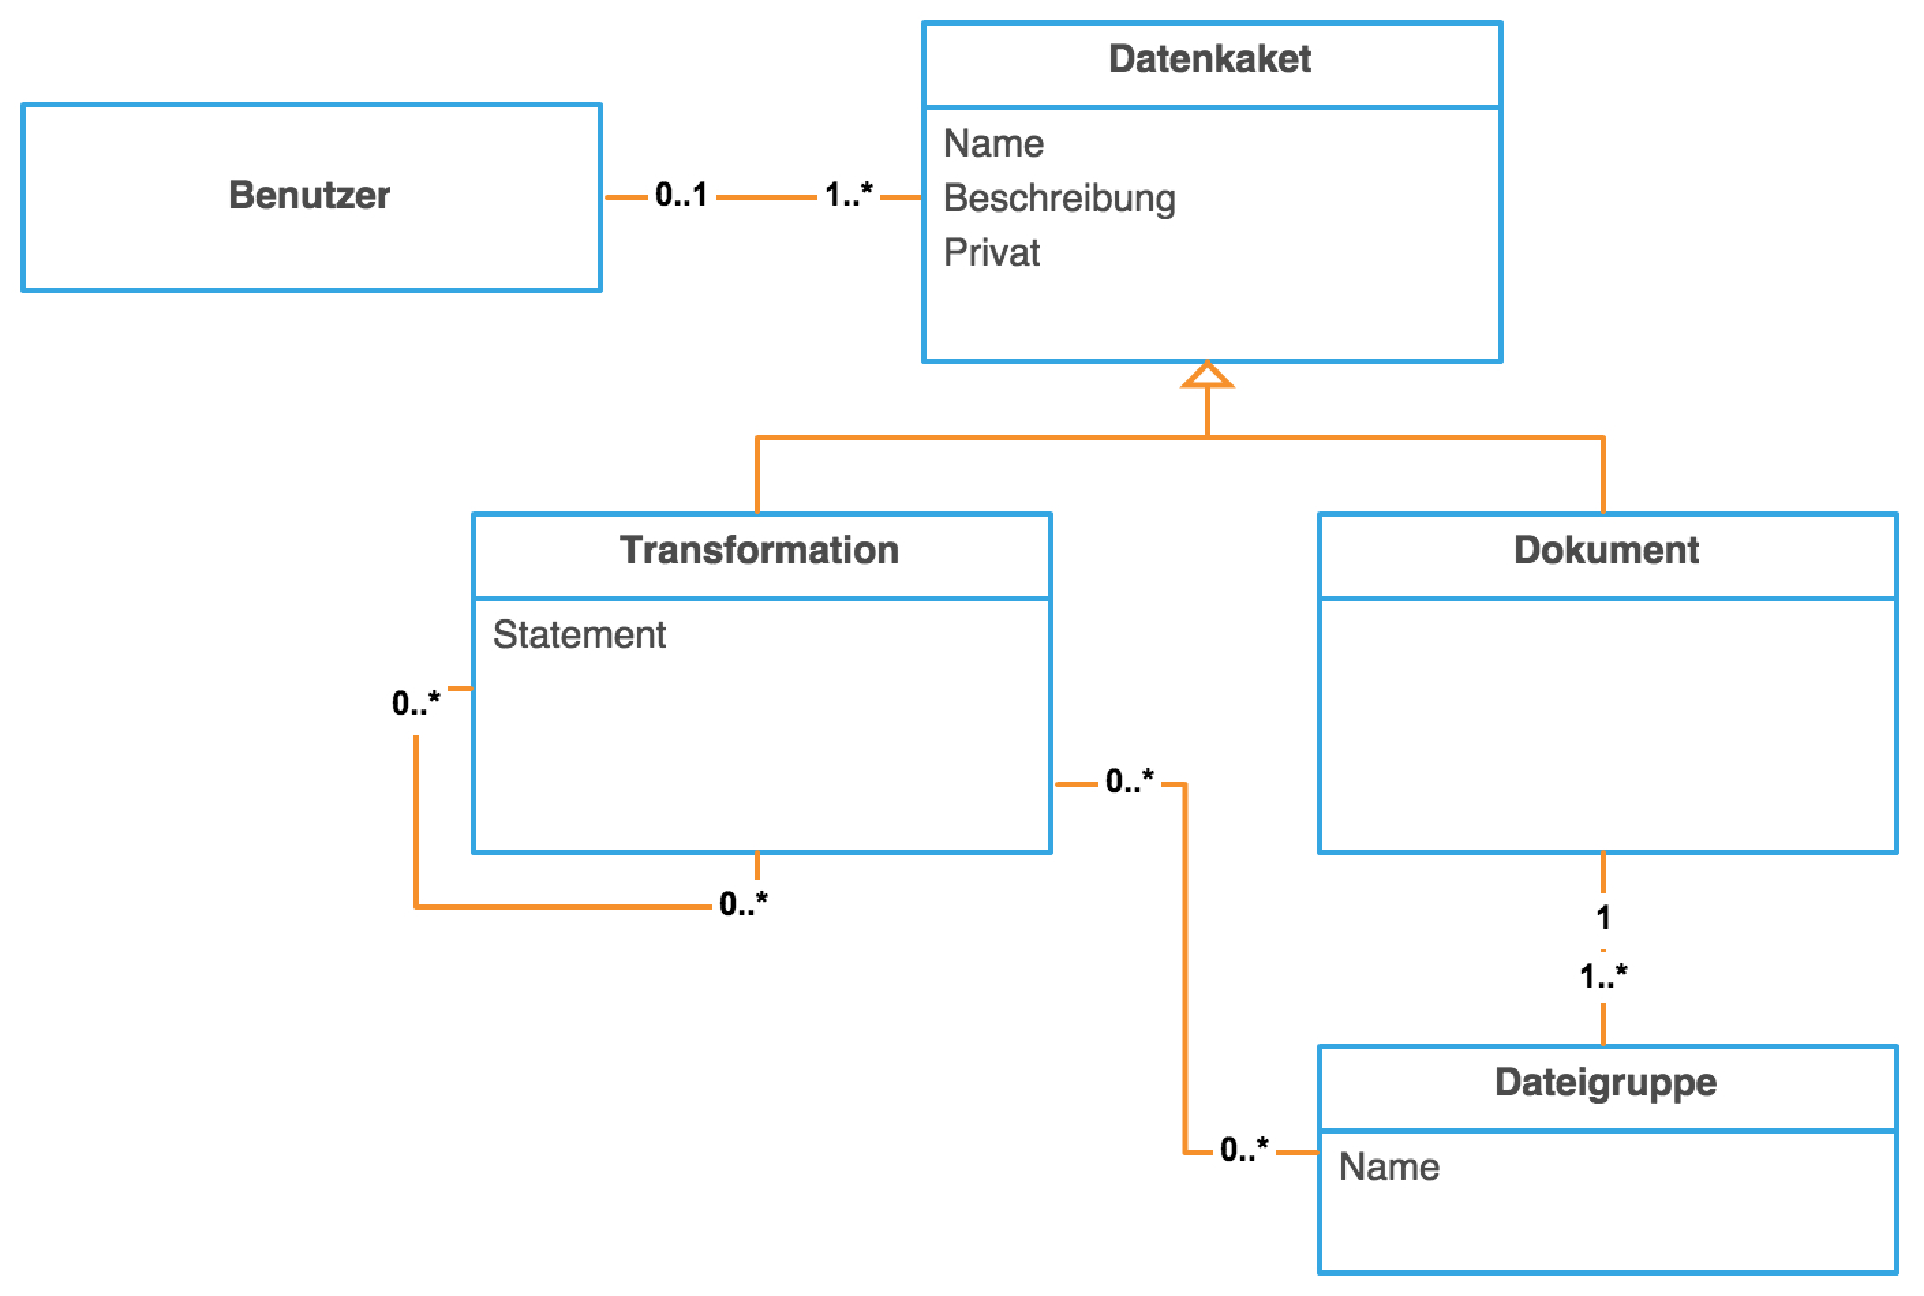
\includegraphics[width=0.8\linewidth]{fig/domain-model.pdf}
    \caption{Domäne OpenDataHub}
    \label{fig:pd:domain-model}
\end{figure}

\section{Dateiformate}

In diesem Abschnitt werden die durch den Kunden gewünschten oder zur Realisierung der Anwendungsfälle in \cref{sec:pd:usecases} benötigten Dateiformate und deren Eigenheiten beschrieben.

\subsection{CSV}
\acf{csv} gilt trotz vielen Schwächen als universellen Austausch/Exportformat für einfache Anwendungsfälle und sollte deshalb zwingend unterstützt werden. Eine \acs{csv} Datei enthält einen Datensatz pro Zeile und die Spalten üblicherweise durch Kommas oder Semikolon getrennt. Die erste Zeile enthält die Namen der einzelnen Felder.

\subsubsection{Erweiterung mit Typen und Geo-Daten}

\gls{geocsv} ist eine durch das Geometa-Lab der HSR spezifizierte Erweiterung der CSV Spezifikation um Geo-Daten mit folgenden Eigenheiten\cite{sfkeller,geocsv,gdal-csv}:

\begin{itemize}
\item Eine optionale Datei mit Endung \path{.csvt} spezifiziert auf einer einzigen Zeile die Datentypen genauer
\item Der spezielle Datentyp ``WKT'' für Geometrien im \gls{wkt} Format
\item Die speziellen Datentypen ``Point(x)'', ``Point(y)'' oder ``CoordX'' bzw. ``CoordY'' für den Spezialfall einer Punktgeometrie
\item Eine optionale Datei mit der Endung \path{.prj} zur Angabe des Referenzsystems, ebenfalls im \gls{wkt} Format\footnote{Achtung, das \path{.prf} Format von ESRI sieht sehr ähnlich aus, enthält jedoch weniger Informationen!}
\item Nur ein Geometrie-Objekt/Spalte pro Datei
\end{itemize}


\subsection{Excel}
Da viele nicht-technische Benutzer mit Microsoft Excel arbeiten\cite{sfkeller} oder Daten im Excel Format anliefern, müssen sowohl der alte Excel 2003 (xls) sowie der neue OpenXML (xlsx) Formate unterstützt werden.

\subsection{GeoJSON}
\gls{geojson} ist eine auf JSON basierende Schema-Spezifikation für Geo-Daten. Dieses Format ist heutzutage weit verbreitet und fast überall wo mit Geo-Daten hantiert wird unterstützt.

\subsection{GeoPackage}
GeoPackage ist ein relativ neues, auf SQLite basiertes, Format. Es ist sehr nahe an SpatiaLite, welches mit Version 4.2 auf GeoPackage wechselt.

\subsection{GML}
\gls{gml} ist ein auf XML basierendes Format für Geo-Daten und ist das Standard-Ausgabeformat von \acs{wfs}-Servern.


\subsection{INTERLIS}
Interlis besteht aus einer Modellbeschreibungssprache und einem Transferformat. Da es praktisch nur in der Schweiz zum Einsatz kommt ist die Unterstützung in kommerzieller Software mässig bis nicht vorhanden.

Interlis existiert in zwei Versionen: Interlis 1 verwendet ein Record-basiertes Transfer-Format, während für Interlis 2 XML gewählt wurde. Mit wenigen Ausnahmen stellt Interlis 2 eine Erweiterung von Interlis 1 um Objekt-orientierte Features dar.

\subsection{KML}
\gls{kml} ist wie \gls{gml} ebenfalls ein auf \gls{xml} basierendes Format, welches in Google Earth Verwendung findet. Speziell bei KML, ist dass es lediglich das Referenzsystem 4326 (klassisches lat/lon) unterstützt.


\subsection{ESRI Shapefile}
Das Shapefile ist ein von der Firma ESRI spezifiziertes Formt zum Austausch von Geo-Daten. Es wird von fast allen Bibliotheken und Systemen unterstützt und eignet sich somit als universelles Austauschformat für Geo-Daten. Das Shapefile wird immer wieder aufgrund dessen Schwächen kritisiert. Da wären beispielsweise die Limitation der Spaltennamen auf 8 Zeichen sowie von Textspalten auf 255 Zeichen. Aus diesem Grund versuchen viele das veraltete Shapefile durch ein moderneres Format wie GeoJSON oder GeoPackage abzulösen\cite{sfkeller}

\subsection{WFS}
Bei \gls{wfs} handelt es sich um einen speziellen Webservice für Geo-Daten. Die Daten können üblicherweise im \gls{gml} Format bezogen werden. Da es sich dabei um einen weit verbreiteten Standard von \gls{ogc} handelt, sollte die Applikation einen direkten Bezug von Daten via einem \acs{wfs} Server ermöglichen.

\subsection{XML}
Da es sich bei \gls{xml} um eine potenziell verschachtelte Datenstruktur handelt, wird vorerst nur eine flache Version ähnlich der von der API von \purl{http://truckinfo.ch} gelieferten in \cref{sec:pd:usecases} beschriebenen Daten. 

\subsection{JSON}
Auch bei JSON handelt es sich um ein Format mit Schachtelungsmöglichkeit. Aus diesem Grund wird auch hier vorerst nur die oberste Ebene betrachtet.


\section{Datenspeicherung}
Ein Ziel dieser Arbeit ist die Erstellung eines Daten-Hubs, welcher es Anbietern ermöglicht, ihre Daten anderen zur Verfügung zu stellen. 

Zur Speicherung der Daten stehen folgende Varianten zur Auswahl.

\subsection{File-basiert}
Die Daten werden direkt im Dateisystem gespeichert. Um Konflikte zwischen Datei-Namen zu vermeiden muss ein Hashing-Schema definiert und verwendet werden. Metadaten zu den Dokumenten werden in einer Datenbank hinterlegt.

Die Daten werden in ihrem Ursprungsformat belassen, bis ein Nutzer eine Transformation auswählt und anwendet. Die Resultate einer solchen Transformation können direkt wieder im Dateisystem zwischengespeichert werden um weitere Abfragen nach der selben Transformation zu beschleunigen.

Die Tatsache, dass die Daten im Dateisystem liegen vereinfacht die Einbindung von Software von Drittanbietern, insbesondere wenn diese Software nur direkt auf Datei-Basis arbeitet (z.B. OGR).

Ein Nachteil dieser Variante ist, dass Cloud-Anbieter wie Heroku keine schreibbaren\cite{herokuReadOnlyFilesystem} bzw. keine beständigen\cite{herokuEphemeralFilesystem} Dateisysteme anbieten, sondern auf die Verwendung von Amazon S3 oder ähnlich verweisen.

Metadaten wie Format oder Original-Dateinamen würden aus Performance-Gründen weiterhin in einer Datenbank gehalten werden.

\subsection{Datenbank-basiert, einzelne Records}\label{sec:pd:datenbank-records}
Die Daten werden in einzelne Records zerlegt und zusammen mit den Metadaten in einer Datenbank gespeichert. Dies erfordert, dass bereits der Daten-Anbieter eine Transformation in das Record-Format auswählen muss. Falls sich herausstellt, dass dies zu langsam ist um es direkt im HTTP-Request des Anbieters durchzuführen, müssen die Daten vor der Transformation zwischengespeichert werden.

Falls die Transformationsresultate zwischengespeichert werden sollen ist eine weitere Datenablage für die Transformationsresultate notwendig.

Die Einbindung von Drittanbieter-Software erfordert mehr Aufwand, falls diese nur auf Dokumenten- oder gar Datei-Ebene arbeiten. In diesem Fall müssen die Daten erst wieder in ein geeignetes Format übersetzt werden, um nach der Transformation wieder in einzelne Records zerlegt zu werden.

\subsection{Datenbank-basiert, Dokument als BLOB}
Die Daten werden ohne Transformation zusammen mit den Metadaten in einer Datenbank abgelegt. Diese Variante hat praktisch alle Vorteile der File-basierten Version.

Falls Dritt-Anbieter-Software nur auf Datei-basis arbeitet kann ein temporäres oder flüchtiges Datei-System verwendet werden.

Für diese Variante existieren folgende Möglichkeiten:
\begin{description}
\item[Daten und Metadaten in der selben Tabelle] Daten und Metadaten werden in der selben Tabelle gespeichert. Dies bietet ein einfacheres Schema, erlaubt jedoch nur ein Daten-Objekt pro Dokument, was ungeeignet ist für Dokument-Typen wie ESRI Shapefiles, welche aus mehr als einer Datei bestehen.
\item[Daten und Metadaten in separaten Tabellen] Daten und Metadaten werden in unterschiedlichen Tabellen gespeichert. Dies erlaubt die Speicherung von Dokumenten bestehend aus mehreren Dateien, oder transformierten Daten als zusätzlichen Daten-Eintrag zu einem Metadaten-Record. Dies erlaubt es auch, Django-Models zu erstellen welche nicht jedes mal die Daten abfragen, obwohl nur Metadaten benötigt werden.
\end{description}

Da File-Formate existieren, welche aus mehr als einer Datei bestehen, ist die Option mit separaten Tabellen vorzuziehen.

\subsubsection{Fazit}
\cref{tab:pd:filestorage-criteria} erläutert die Kriterien für die Bewertung der verschiedenen Varianten.
\mytable{lXc}{
  \textbf{Kriterium} & \textbf{Beschreibung} & \textbf{Gewichtung} \\
  \midrule
  \textbf{Original bleibt erhalten} & Das Original-Dokument bleibt erhalten oder kann komplett rekonstruiert werden. Dies bietet folgende Vorteile: Verbesserungen an der Software (Parser) zeigt auch bei alten Daten Wirkung, ausserdem gehen keine Daten verloren durch den Upload. & \threeOfThree \\
  \textbf{Einbindung Software} & Erlaubt die Einbindung von Drittanbieter-Software. Dies ist möglich auf File-basis, oder direkt als Memory Buffer, falls Python-Code aufgerufen wird. & \oneOfThree \\
  \textbf{Beliebige Formate} & Die Variante unterstützt beliebige Formate. Anschliessende Transformationen können nur auf bekannte Formate angewandt werden, aber auch unbekannte Formate können gespeichert und zum Download angeboten werden. Die Daten können verwendet werden, falls später ein Parser geschrieben wird für das bisher unbekannte Format. & \twoOfThree \\
  \textbf{Cloud} & Cloud-Anbieter wie Heroku bieten oft kein permanentes File-System, sondern verweisen auf Storage Provider wie Amazon S3 oder auf Datenbanken als Daten-Speicher. Unterstützung für Cloud-Anbieter ist kein zwingendes Kriterium für diese Arbeit, soll aber falls möglich erhalten bleiben. & \oneOfThree \\
}{Bewertungskriterien Datenspeicherung}{pd:filestorage-criteria}

\cref{tab:pd:transformation-lang-results} fasst die verschiedenen Optionen zusammen.
\mytable{lXXX}{
  \textbf{Kriterium} & \textbf{File} & \textbf{DB: Record} & \textbf{DB: Schhemalos} \\
  \midrule
  \textbf{Original bleibt erhalten} & \threeOfThree & \oneOfThree & \threeOfThree \\
  \textbf{Einbindung Software} & \threeOfThree & \twoOfThree & \threeOfThree \\
  \textbf{Beliebige Formate} & \threeOfThree & \oneOfThree & \threeOfThree \\
  \textbf{Cloud} & \twoOfThree & \threeOfThree & \threeOfThree \\
  \midrule
  \textbf{Total} & \threeOfThree & \oneOfThree & \threeOfThree \\
}{Auswertung verschiedener Speicher-Varianten}{pd:filestorage-results}

\begin{decision}[label=dec:pd:datenspeicherung]{Datenspeicherung}
Aus Gründen der Kompatibilität zu Cloud-Anbietern, insbesondere Heroku ohne gleich Cloud-Datenspeicher wie Amazon S3 verwenden zu müssen, wurde bereits früh entscheiden, die Dateien in der Datenbank zu persistieren. Da die Datenhaltung ohnehin eine sehr lose Kopplung zur restlichen Applikation besitzen soll, kann künftig auch eine andere Strategie implementiert werden.
\end{decision}

\section{Intermediäres Format}

Bei $N$ Dateiformaten würden bei 1-zu-1 Format-Konversionen bereits $\frac{N*(N-1)}2$ Übersetzungsmodule benötigt, um lediglich zwischen den Dateiformaten zu konvertieren. Zudem muss es möglich sein das Schema der Daten zu transformieren. Diese Tatsache erfordert zwingend ein intermediäres, einheitliches Format ohne welches eine generische Transformation unmöglich wäre.

In diesem Abschnitt werden diverse Optionen im Hinblick auf deren Vor- und Nachteile sowie Eignung beschrieben. 

\subsection{Datenbank}
Bei dieser Variante wäre das Intermediäre Format äquivalent der Datenspeicherung wie sie in \cref{sec:pd:datenbank-records} beschrieben ist. Die Daten würden aber dennoch separat als Originaldateien abgelegt werden um keine Informationen zu vernichten. Der grosse Vorteil dieser Variante ist, dass die Transformationen dann mittels SQL Abfragen auf die diversen Datenbanktabellen erfolgen kann. Man ist dabei jedoch auf die Funktionalität der Datenbank limitiert und kann nur sehr schlecht Transformationen anbieten die dessen Fähigkeiten übersteigen.

\xxx[Braucht noch Anmerkungen zu Performance, weil unten nur 1 von 3 Sternen vergeben wurde. Verluste in in Konversion Python -> SQL/SQL -> Python sind evtl. nicht offensichtlich - dies wird erst in der nächsten Section erwähnt.]

\subsection{ogrtools}

Ogrtools ist eine Python-Implementation des \acs{cli}-Tools ``ogr2ogr'' erweitert mit simplen Transformationen. Ogr2ogr wie auch ogrtools verwenden die kompilierten OGR/GDAL Bibliotheken, welche 1-zu-1 (ogr $\to$ ogr) Format-Transformationen ermöglichen. Beispielsweise können ESRI Shapefiles (.shp) in \gls{kml} oder \gls{gml} Dateien umgewandelt werden. Da die Formate untereinander nicht immer kompatibel sind kann es durchaus zum Verlust von Informationen kommen.

Sollte die ogrtools Bibliothek verwendet werden, so würde auf der existierenden Transformationssprache bzw. Tranformationskonfiguration aufgebaut und dieses um weitere Operationen wie beispielsweise Filterung oder Joins erweitert. Eine ogrtools Beispielskonfiguration \cite[README, ogrtransform library]{ogrtools} ist in \cref{src:pd:ogrtools} zu sehen.


\begin{srclst}[label=src:pd:ogrtools]{json}{ogrtools Mapping-Konfiguration}
{
  "//": "OGR transformation configuration",
  "src_format": "Interlis 2",
  "dst_format": "PostgreSQL",
  "dst_dsco": {},
  "dst_lco": {
    "SCHEMA": "public"
  },
  "layers": {
    "roadsexdm2ben_roads_streetnameposition": {
      "fields": {
        "tid": {
          "src": "TID",
          "type": "String"
        },
        "street": {
          "src": "Street",
          "type": "String"
        },
        "namori": {
          "src": "NamOri",
          "type": "Real"
        }
      },
      "geometry_type": "Point",
      "src_layer": "RoadsExdm2ben.Roads.StreetNamePosition",
      "geom_fields": {
        "nampos": {
          "src": "NamPos",
          "type": "Point"
        }
      }
    },
    "roadsexdm2ben_roads_streetaxis": {
      "fields": {
        "tid": {
          "src": "TID",
          "type": "String"
        },
        "street": {
          "src": "Street",
          "type": "String"
        }
      },
      "geometry_type": "MultiLineString",
      "src_layer": "RoadsExdm2ben.Roads.StreetAxis",
      "geom_fields": {
        "geometry": {
          "src": "Geometry",
          "type": "MultiLineString"
        }
      }
    }
  }
  "..."
}
\end{srclst}

\subsection{Python Tabellenstrukturen}

\subsubsection{Petl}
Petl\footnote{http://petl.readthedocs.org/} ist eine Python \acs{etl} Bibliothek. Petl erlaubt es diverse Formate in eine Tabellenstruktur zu laden und bietet ein \acs{api} um darauf diverse Transformationen anzuwenden oder gar ganze Transformations-Pipelines aufzusetzen.

Der Vorteil von petl gegenüber anderen Lösungen liegt in dessen ``Lazy evaluation''. Es werden keine Daten geladen oder transformiert, bis das Resultat benötigt wird. Dann erst werden die Daten Zeile für Zeile eingelesen und durch die Transformations-Pipeline geschleust. Petl kann somit mit sehr grossen Datenmengen umgehen, ist aber im vergleich zur Konkurrenz langsamer und für Performance-kritische Applikationen ungeeignet \cite[Intro $\to$ Design goals]{petl}.


\subsubsection{Pandas}
Pandas ist zwar eine Bibliothek zur Datenanalyse, sozusagen das ``R'' für Python. Doch die zugrundeliegenden, ebenfalls Tabellen-artigen Datenstrukturen zusammen mit der \acs{api} von Pandas macht Transformationen wie Joins, Filtern, Umbenennungen und Berechnungen sowie String-Operationen sehr einfach. Pandas baut auf NumPy auf, der de-facto Standardbibliothek für Matrizen/Berechnungen in Python. Da NumPy in C bzw. Fortran und das Python \acs{api} sehr funktional-orientiert implementiert sind, lassen sich Operationen auf ganze Spalten oder Tabellen anwenden, was zu einer für Python-Verhältnisse sehr hohen Performance führt.


\begin{srclst}[label=src:pd:geopandas]{pycon}{Pandas mit GeoPandas}
>>> import geopandas
>>> gdf = geopandas.GeoDataFrame.from_file('Bahnhoefe.shp')
>>> gdf.columns
Index([u'CNTRYNAME', u'CONURB', u'DUP_NAME', u'LEVEL', u'NAME', u'NATION', u'PROV1NAME', u'TYPE', u'geometry'], dtype='object')
}
>>> gdf.CONURB[:10]
0         None
1      Chiasso
2      Balerna
3    Mendrisio
4     Capolago
5     Capolago
6     Capolago
7     Capolago
8     Capolago
9     Maroggia
>>> gdf[gdf.CONURB == 'Zürich'][:5]
        CNTRYNAME  CONURB DUP_NAME  LEVEL                  NAME  NATION  \
1317  Switzerland  Zürich        N     10     Sood Oberleimbach      41
1346  Switzerland  Zürich        N     10       Zürich Leimbach      41
1360  Switzerland  Zürich        N     10        Zürich Mannegg      41
1373  Switzerland  Zürich        N     10    Zürich Wollishofen      41
1374  Switzerland  Zürich        N     10  Zürich Tiefenbrünnen      41

     PROV1NAME  TYPE                                     geometry
1317    Zürich    30  POINT (681918.8961174991 241523.9264312923)
1346    Zürich    30  POINT (681750.8866669014 243289.5358952266)
1360    Zürich    30  POINT (681746.1775964648 244178.9977101207)
1373    Zürich    30  POINT (682765.2814791016 244804.6936600676)
1374    Zürich    30  POINT (685054.0860048197 244870.4588255175)
>>> gdf[gdf.geometry.within(shapely.geometry.Polygon([(704940,231559), (704949,231559),(704945,231550),]))]
        CNTRYNAME      CONURB DUP_NAME  LEVEL        NAME  NATION   PROV1NAME  \
1196  Switzerland  Rapperswil        N     10  Rapperswil      41  Ostschweiz

      TYPE                                     geometry
1196    30  POINT (704945.8093275279 231556.7192434487)
\end{srclst}


\subsubsection{PyTables/HDF}
PyTables ist eine high-performance Python-Bibliothek die wie Pandas ebenfalls auf NumPy aufbaut. Da das \acs{api} von PyTables im Vergleich zu Pandas eher low-level ist und weniger bietet wurde diese Bibliothek nicht weiter verfolgt.

\subsection{Fazit}

\cref{tab:pd:format-criteria} erläutert die wichtigsten Kriterien für die Bewertung der beschriebenen Lösungen.

\mytable{lXc}{
  \textbf{Kriterium} & \textbf{Beschreibung} & \textbf{Gewichtung} \\
  \midrule
  \textbf{Performance} & Wie performant ist die Lösung. Wichtig aufgrund des Effizienz \acs{nfr} welches beim Treffen mit Herrn Dorfschmid geäussert wurde. & \twoOfThree \\

  \textbf{Machbarkeit} & Die generelle Umsetzbarkeit der funktionalen Anforderungen mit dieser Lösung. & \threeOfThree \\

  \textbf{Aufwand / Komplexität} & Der benötigte Aufwand um Applikation der Lösung umzusetzen. & \twoOfThree \\

}{Bewertungskriterien Intermediäres Format}{pd:format-criteria}


\cref{tab:pd:format-results} fasst die verschiedenen Optionen zusammen.
\mytable{lXXXXX}{

  \textbf{Kriterium} & \textbf{Datenbank} & \textbf{ogrtools} & \textbf{Petl} & \textbf{Pandas} & \textbf{PyTables} \\

  \midrule

  \textbf{Performance} & \oneOfThree & ? & \oneOfThree & \twoOfThree & \oneOfThree \\

  \textbf{Machbarkeit} & \twoOfThree & \oneOfThree & \twoOfThree & \threeOfThree  & \twoOfThree \\

  \textbf{Aufwand / Komplexität} & \twoOfThree & \oneOfThree & \twoOfThree & \twoOfThree & \oneOfThree \\

  \midrule

  \textbf{Total} & \twoOfThree & \oneOfThree & \twoOfThree & \threeOfThree & \twoOfThree \\
}{Auswertung verschiedener Format-Varianten}{pd:format-results}


\begin{decision}[label=dec:pd:format]{Intermediäres Format}
Aufgrund der sowohl mächtigen \acs{api} wie auch der gleichzeitig hohen Performance und Integration mit Geo-Daten bzw. Shapely wurde für Pandas und deren Datenstrukturen entschieden. Die Variante in der Datenbank wurde obschon der Aufwand für die Transformationen komplett entfallen würde, aufgrund der Machbarkeit im Zusammenhang mit Echtzeit-Datenquellen verworfen.
\end{decision}

\section{Transformation}

\subsection{Anforderungen}
\xxx{gehört das wirklich hier hin? @chuesler}

Folgende Daten-Arten sind zu unterscheiden:
\begin{itemize}
\item Tabellarische Daten (z.B. CSV, Excel)
\item Baum-artige Daten (z.B. XML)
\item Unstrukturierte Daten (z.B. Bilder, unstrukturierter Text)
\end{itemize}

Diese Arbeit befasst sich aus Zeitgründen nur mit tabellarischen Daten.

In \cref{tab:pd:transformation-lang-req} werden die Anforderungen an die Transformations-Sprache zusammengefasst.

\mytable{lX}{
  \textbf{Anforderung} & \textbf{Beschreibung}\\
  \midrule
  \textbf{Mapping} & Felder müssen 1:1 auf andere Felder gemappt werden können (Feld umbenennen) \\
  \textbf{Default-Werte} & Neue Felder mit Default-Werten müssen hinzugefügt werden können \\
  \textbf{Joins} & Mehrere Datenquellen müssen miteinander verknüpft werden können. Dabei muss immer eine Join-Bedingung angegeben werden (keine karthesischen Produkte) \\
  \textbf{Filter/Prädikate} & Daten sollen gefiltert werden können \\
  \textbf{Erweiterbare Operationen} & Es sollen neue Operationen definiert werden können (in Python) \\
  \textbf{Sortierung} & Das Resultat der Transformation soll sortiert werden können\\
}{Anforderungen an die Transformations-Sprache/Konfiguration}{pd:transformation-lang-req}

\subsection{Datenbank-basiert: SQL}
Die Daten werden in einer Datenbank gespeichert, dort transformiert, und wieder herausgelesen.

Vorteile dieser Variante sind, dass die Abfrage-Sprache bereits vorhanden und bekannt ist und dass je nach verwendeter Datenbank auf vorhandene Funktionen und Optimierungen zurückgegriffen werden kann. Falls Postgres mit PostGIS zum Einsatz kommt, kann auch im Geo-Bereich eine umfassende Funktions-Bibliothek verwendet werden. 

Da die Daten jedoch vor der Transformation geparst, und anschliessend wieder formatiert werden müssen, entsteht ein beträchtlicher Performance-Verlust alleine durch das Abspeichern und Auslesen der Daten. Hinzu kommt, dass grosse Performance-Vorteile durch z.B. durch Indizes, nicht realisiert werden können, da nur eine einmalige Transformation stattfindet und daher die Kosten für die Erstellung des Indexes nicht amortisiert werden.

\subsection{ogrtools: ogrtransform}
Ogrtools beinhaltet bereits eine Transformations-Konfiguration namens ogrtransform. Aktuell werden aber diverse der gewünschten Features nicht unterstützt, wie z.B. Joins oder Filter. Ausserdem basiert die Implementation auf ogr2ogr, was die Daten-Arten, auf welche Transformationen angewendet werden können, massiv limitiert.

Da ogr2ogr nur auf Datei-Basis arbeitet, müssen die Daten, falls sie nicht in einem von ogr2ogr unterstützten Format vorliegen, erst geparst und formattiert und anschliessend ins Datei-System geschrieben werden. Nach der Transformation muss das Resultat wieder geparst werden, um in das vom Benutzer gewünschte Format konvertiert werden zu können. 

\subsection{DSL: Vereinfachtes SQL}
Dieses Format lehnt sich an SELECT aus SQL an. Es ist anzunehmen, dass Experten im Bereich Datentransformation sich mit SQL auskennen, was das Erlernen dieser Query-Sprache sehr vereinfachen würde. Dies wurde durch \prof bestätigt. \xxx[\prof rausnehmen?]

Da als Backend nicht eine SQL-Datenbank verwendet wird, sondern die Operationen auf Pandas DataFrames übersetzt werden, sind einige kleinere Differenzen zu SQL unvermeidbar. Zur Performance von Joins mit Pandas DataFrame, siehe \cite{pandasMergePerformance}.

Neue Funktionen können in Python definiert werden.

\subsection{DSL: Eigenes Format}
Diese Variante besitzt grundsätzlich die selben Eigenschaften wie eine SQL-basierte DSL. Dieser gegenüber entfällt jedoch das Familiaritäts-Argument. Ausserdem muss eine passende, einfach zu erlernende Syntax definiert werden.

\subsection{Fazit}
\cref{tab:pd:transformation-lang-criteria} erläutert die Kriterien für die Bewertung der verschiedenen Varianten.
\mytable{lXc}{
  \textbf{Kriterium} & \textbf{Beschreibung} & \textbf{Gewichtung} \\
  \midrule
  \textbf{Features} & Bereits vorhandene Unterstützung für die in \cref{tab:pd:transformation-lang-req} aufgelisteten Features & \oneOfThree \\
  \textbf{Geo-Daten} & Unterstützung für Geo-Daten & \threeOfThree \\
  \textbf{Allgemeine Daten} & Unterstützung für Nicht-Geo-Daten & \threeOfThree \\
  \textbf{Performance} & Performance der Transformation. Da diese Arbeit vor allem als Prototyp dienen soll ist dies nicht erste Priorität, soll aber auch nicht komplett Vernachlässigt werden. & \oneOfThree \\
  \textbf{Funktionen} & Erweiterbarkeit um eigene bzw. benutzerdefinierte Funktionen (in externer Sprache) & \twoOfThree \\
  \textbf{Familiarität} & Wie gut kennen Experten auf dem Gebiet Datentransformation diese Sprache, bzw. wie viel Lernaufwand ist notwendig, um die Sprache zu erlernen & \oneOfThree \\
}{Bewertungskriterien Transformationssprache}{pd:transformation-lang-criteria}
\xxx[Gewichtung der Kriterien abstimmen zwischen einzelnen Bereichen]
\cref{tab:pd:transformation-lang-results} fasst die verschiedenen Optionen zusammen.
\mytable{lXXXX}{
  \textbf{Kriterium} & \textbf{Datenbank: SQL} & \textbf{ogrtransform} & \textbf{DSL: SQL} & \textbf{DSL: Eigenes Format} \\
  \midrule
  \textbf{Features} & \threeOfThree & \oneOfThree & \threeOfThree & \threeOfThree \\
  \textbf{Geo-Daten} & \threeOfThree & \threeOfThree & \threeOfThree & \threeOfThree\\
  \textbf{Allgemeine Daten} & \threeOfThree & \oneOfThree & \threeOfThree & \threeOfThree\\
  \textbf{Performance} & \oneOfThree & \oneOfThree & \twoOfThree & \twoOfThree \\
  \textbf{Funktionen} & \twoOfThree & \oneOfThree & \threeOfThree & \threeOfThree \\
  \textbf{Familiarität} & \threeOfThree & \oneOfThree & \threeOfThree & \oneOfThree \\
  \midrule
  \textbf{Total} & \twoOfThree & \oneOfThree & \threeOfThree & \twoOfThree \\
}{Auswertung verschiedener Transformations-Sprachen}{pd:transformation-lang-results}
\xxx[@chuesler irgendwie überlappen die intermediäres format und sprache zu sehr. wo gehören z.B. performance und geo-daten hin? geht es hier nur um die sprache oder auch um die implementation dessen?]
Aufgrund dieser Auswertung fällt die Wahl auf eine SQL-basierte DSL.

\section{Frontend}
\subsection{Technologie}
\begin{decision}[label=dec:frontend:technology]{AngularJS als Frontendtechnologie}
Da \chuf und \fscf schon viel Erfahrung mit AngularJS gesammelt haben und dies ein sehr etabliertes Framework ist, haben wir uns für dieses entschieden. Evaluiert wurde es bereits im Rahmen den Studienarbeiten von \fscf und \rlif.
\end{decision}
\subsection{Bootstrap}
\mytable{lXXX}{

  \textbf{Kriterium} & \textbf{Bootstrap} & \textbf{Foundation} & \textbf{UIkit} \\

  \midrule

  \textbf{Bekanntheit} & \threeOfThree & \oneOfThree & \oneOfThree \\

  \textbf{Anz. Elemente} & \twoOfThree & \twoOfThree & \twoOfThree  \\

  \textbf{AngularJS} & \threeOfThree & \oneOfThree & \twoOfThree  \\

  \midrule

  \textbf{Total} & \threeOfThree & \oneOfThree & \twoOfThree  \\
}{Auswertung diverser Frontend Frameworks}{pd:frontend-bootstrap-results}
\begin{decision}[label=dec:frontend:bootstrap]{Bootstrap als Designgrundlage}
Aufgrund der Evaluation verschiedener Framework und der Vertrautheit mit Bootstrap, haben wir uns für die Verwendung von Twitter Bootstrap entschieden. Das Layout wird an Twitter Bootstrap angelehnt.
\end{decision}


\subsection{Menupunkte}
Die Menuführung soll schlicht und übersichtlich gehalten werden. Der Prototyp umfasst folgende Struktur: Daten - Daten bereitstellen - Transformation erstellen. \\
Unter dem Menupunkt Daten werden bestehende Dokumente und Transformationen bereitgestellt.\\

\subsection{Assisstent}
Es kann sich schwierig gestalten, eine Transformation von Grund auf zu erstellen. Deshalb soll eine Art Assistent zur Verfügung gestellt werden, welcher ein initiales ODHQL Query erstellen kann. Dieser soll Queries mit JOIN und UNION Operationen erstellen können.

\subsection{Drafts}
\begin{figure}[H]
    \centering
    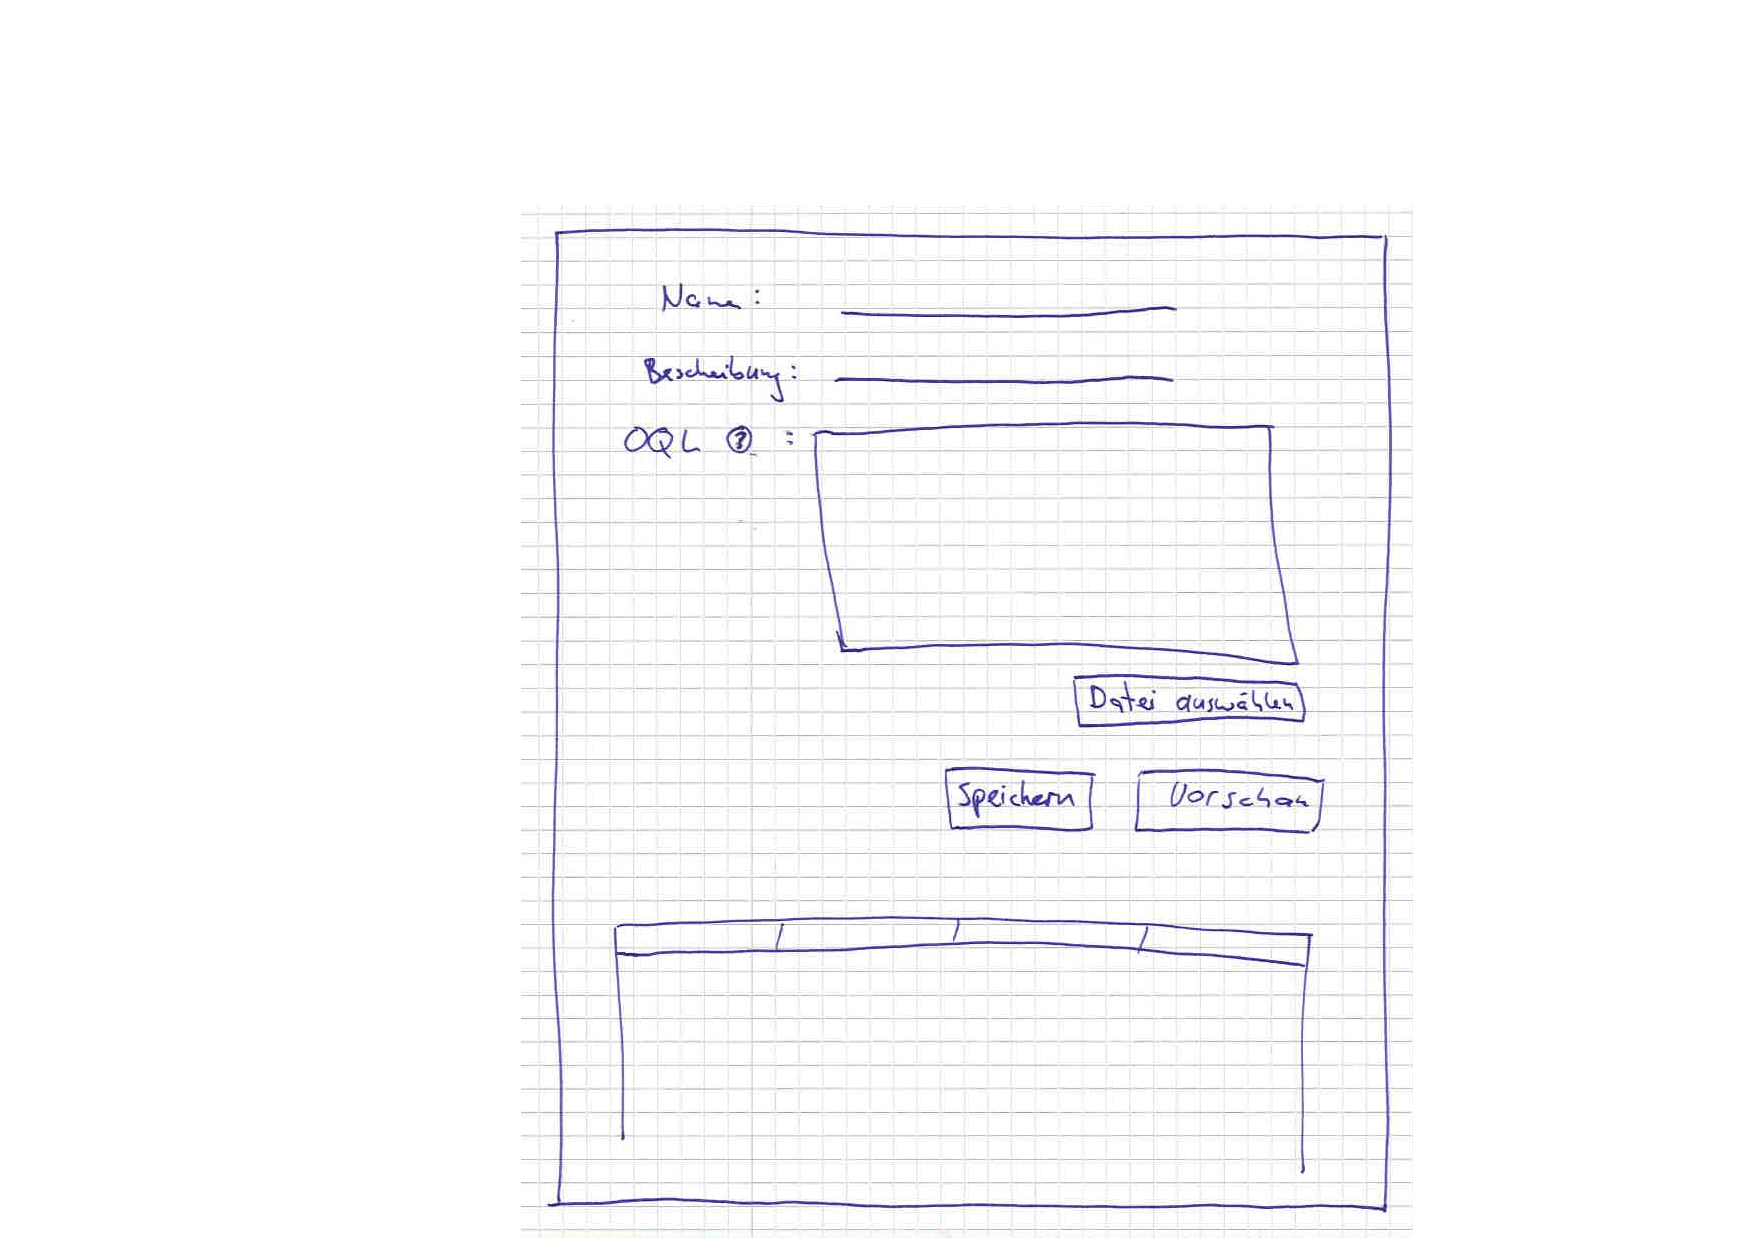
\includegraphics[width=0.6\linewidth]{fig/mockup_hcdi}
    \caption{Frühes Mockup ``Transformation erstellen''}
    \label{fig:pd:mockup-upload}
\end{figure}
\begin{figure}[H]
    \centering
    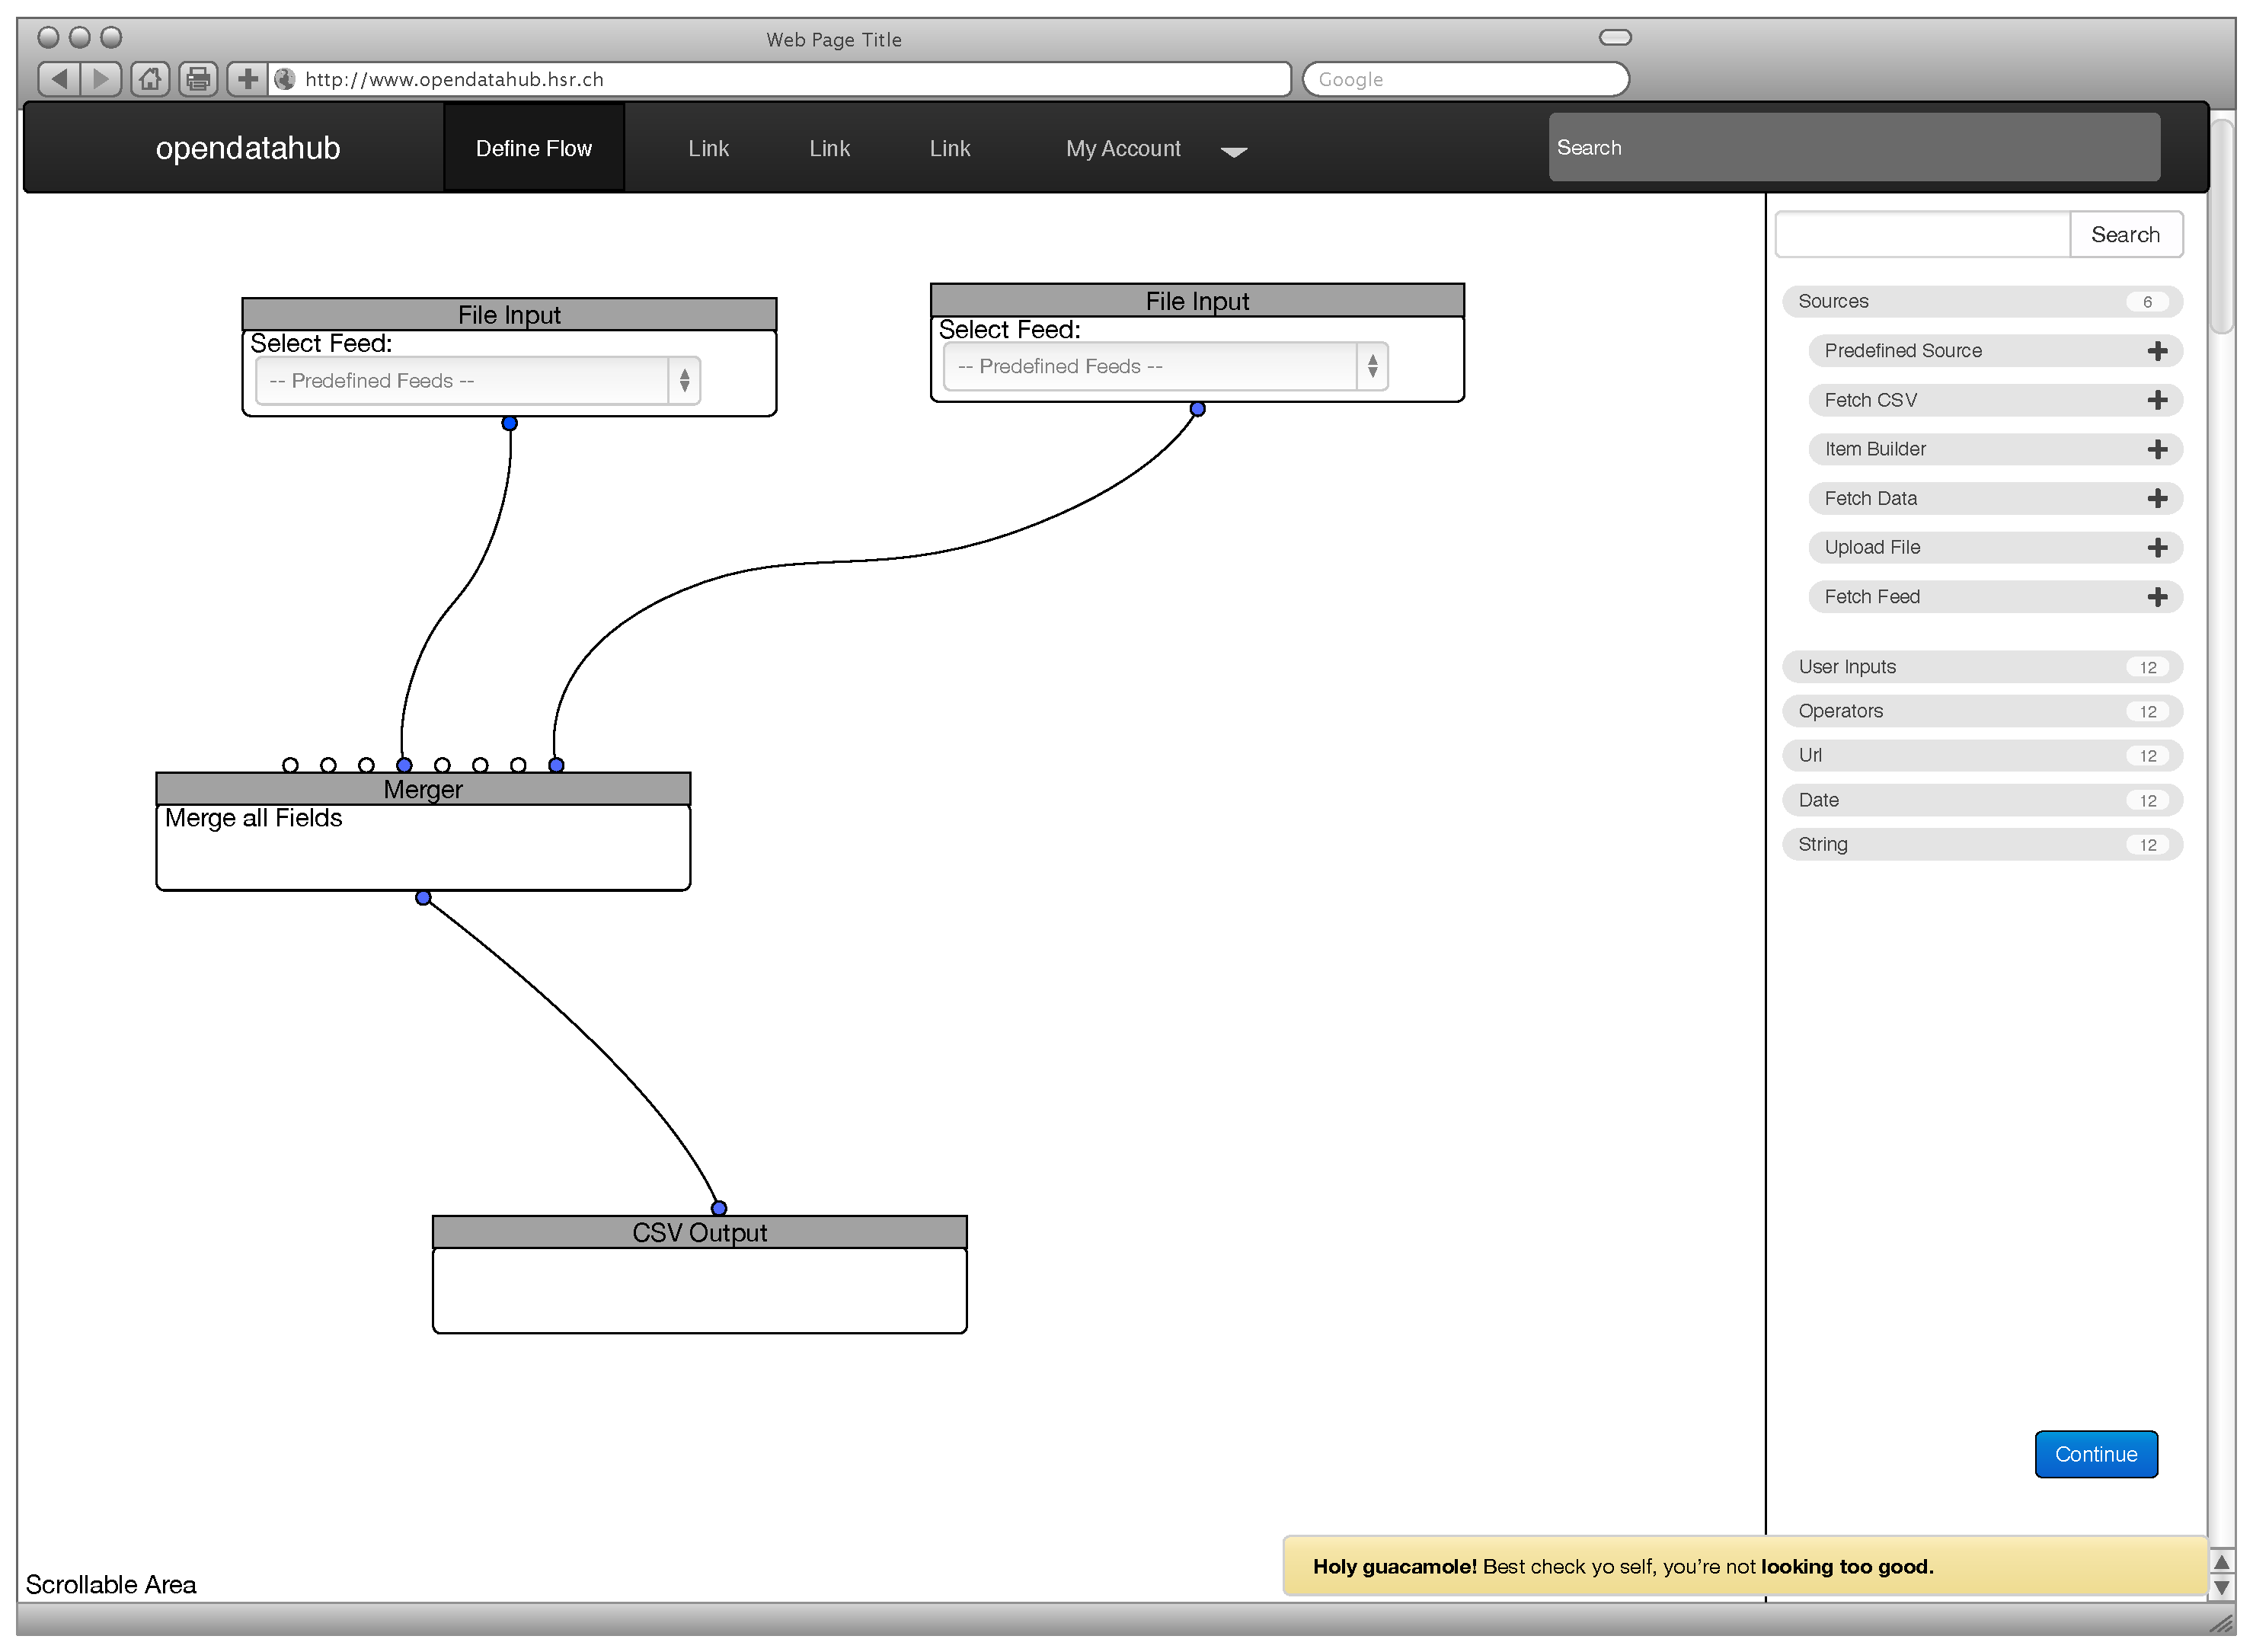
\includegraphics[width=0.8\linewidth]{fig/Wireframes-Connectors}
    \caption{Frühe Idee Transformation mit ``Pipes'' erstellen. (Verworfen)}
    \label{fig:pd:connectors}
\end{figure}
\begin{figure}[H]
    \centering
    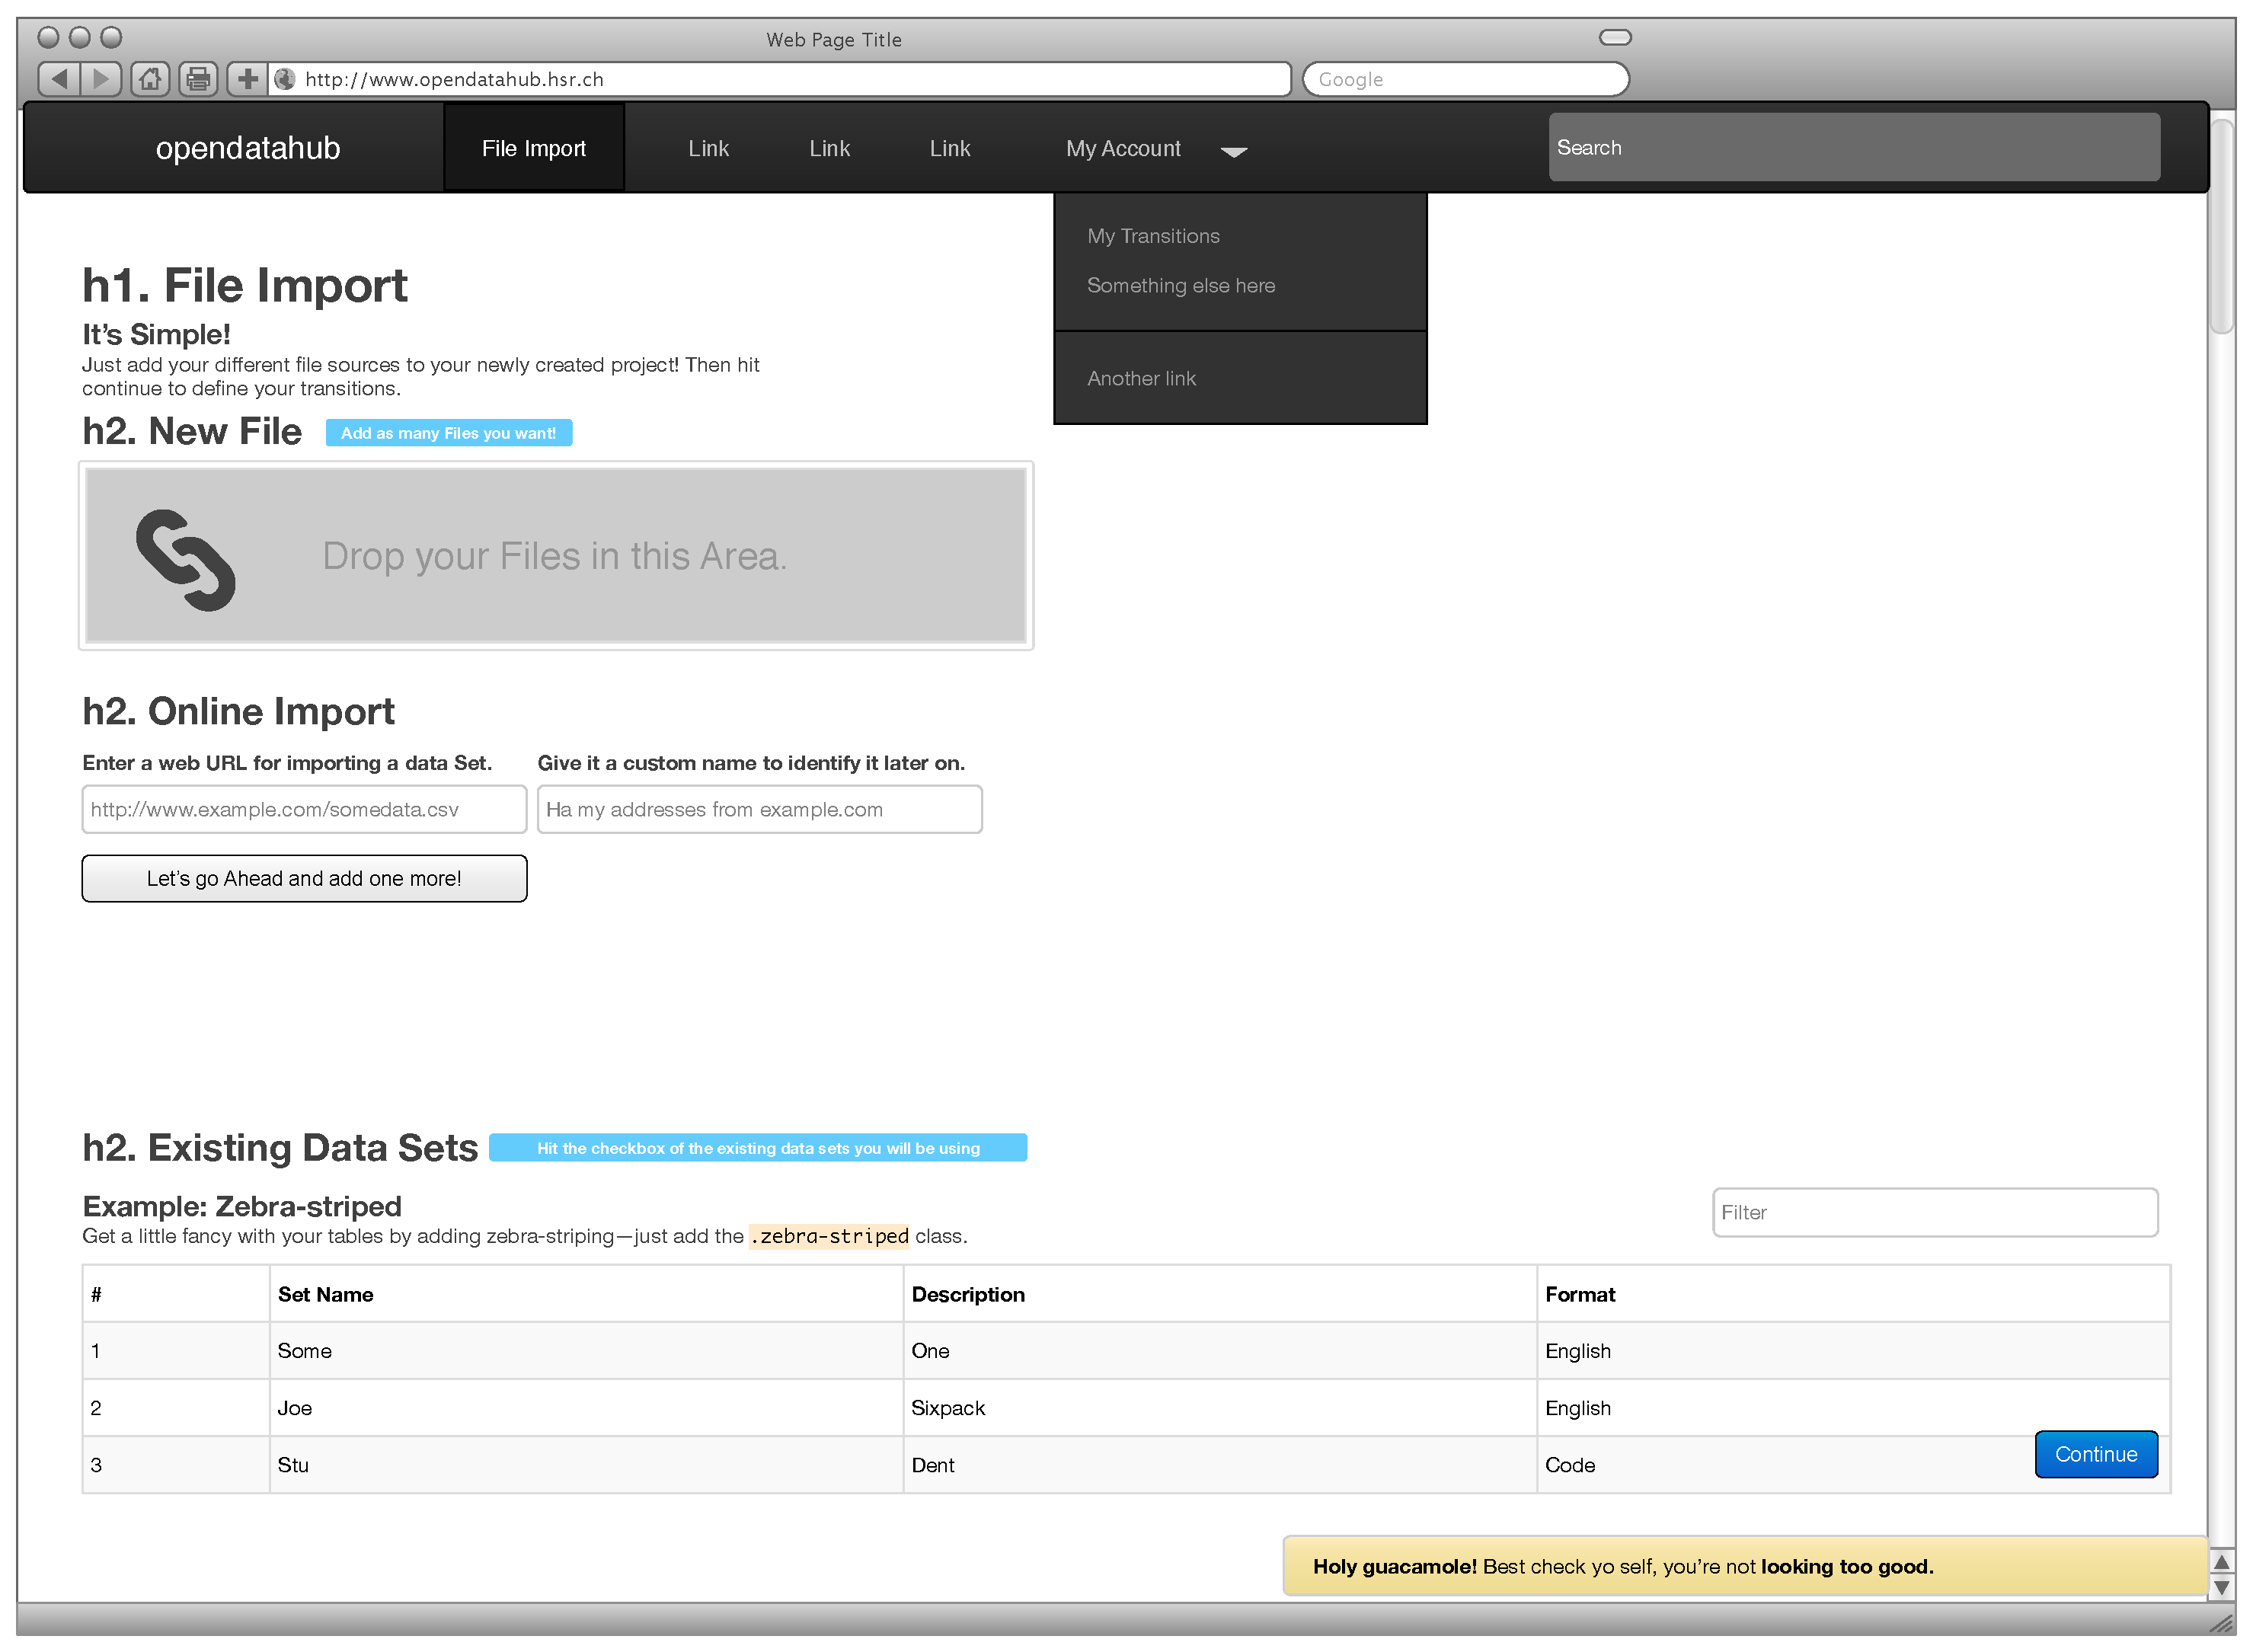
\includegraphics[width=0.8\linewidth]{fig/Wireframes-Upload}
    \caption{Frühes Mockup für Upload Formular}
    \label{fig:pd:wireframe-upload}
\end{figure}